
%(BEGIN_QUESTION)
% Copyright 2011, Tony R. Kuphaldt, released under the Creative Commons Attribution License (v 1.0)
% This means you may do almost anything with this work of mine, so long as you give me proper credit

Anta at vi injiserer samme mobile fase i to ulike kolonner, hver med ulik tetthet av stasjonærfasemateriale ("pakking"):

$$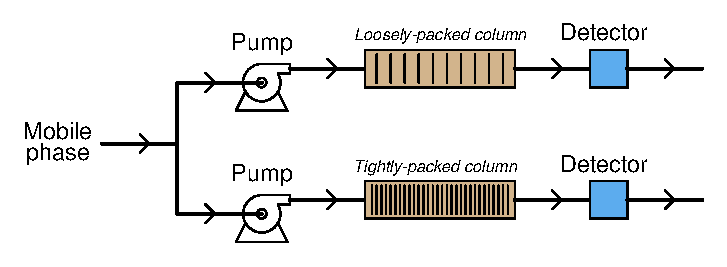
\includegraphics[width=15.5cm]{i00667x01.eps}$$

Hvis alle andre faktorer er like, hvilken kolonne vil gjøre en bedre jobb med å separere ulike komponenter i den mobile fasen (altså ulike kjemiske stoffer blandet i samme prøve)? Hvilken kolonne vil gjøre separasjonen {\it raskere}?

\vskip 20pt \vbox{\hrule \hbox{\strut \vrule{} {\bf Forslag til sokratisk diskusjon} \vrule} \hrule}

\begin{itemize}
\item{} Kromatografi kan sammenlignes med et maratonløp, der grupper av løpere blir mer separert over tid på grunn av ulike hastigheter. Ved slutten av løpet er det lett å identifisere hvem som er raske, hvem som er sakte, og hvor mange av hver type som var med fra start. Relater sammenligningen av to kolonner til maratonanalogien: hva representerer en tettpakket kolonne versus en løst pakket kolonne?
\item{} En viktig variabel som påvirker retensjonstiden til et stoff i en kromatografkolonne er {\it temperatur}. Forklar hvordan økt kolonnetemperatur påvirker forplantning av en {\it gassformig} forbindelse. Forklar deretter hvordan økt kolonnetemperatur påvirker forplantning av en {\it flytende} forbindelse.
\item{} Identifiser andre variabler som påvirker retensjonstiden til en forbindelse i en kromatografkolonne, utover pakningstetthet.
\end{itemize}

\underbar{file i00667no}
%(END_QUESTION)





%(BEGIN_ANSWER)


%(END_ANSWER)





%(BEGIN_NOTES)

Den tettpakkede kolonnen vil separere komponentene bedre, men det vil ta lengre tid.

\vskip 10pt

Endringer i kolonnetemperatur påvirker væskeviskositet. For gasser {\it øker} viskositeten ved økt temperatur, slik at forbindelsen flyter saktere. For væsker gir økt temperatur vanligvis {\it lavere} viskositet, slik at forbindelsen flyter raskere.

%INDEX% Måling, analytisk: kromatografi

%(END_NOTES)
